
\section*{Comunicazioni digitali}


\begin{adjustwidth*}{-2.3cm}{-2cm}
    \begin{center}
        \tikzsetnextfilename{digital_channel}
        \documentclass{standalone}

\usepackage{tikz,pgf} %and any other packages or tikzlibraries your picture needs

\usepackage{pgfplots}
\usepackage[letterpaper,top=2cm,bottom=2cm,left=2cm,right=2cm,marginparwidth=1.75cm]{geometry}
\usepackage{mathtools} 
\usepackage{forest}
\usepackage{standalone}
\usepackage{pgfplots}
\usepackage{graphicx}
\usepackage{svg}
\usepackage{array}
\usepackage{pgfplots}
\usepackage{tikz}
\usepackage[utf8]{inputenc}
\usepackage[colorlinks=true, allcolors=blue]{hyperref}
\usetikzlibrary{positioning, arrows.meta, fit, shapes}
\begin{document}


 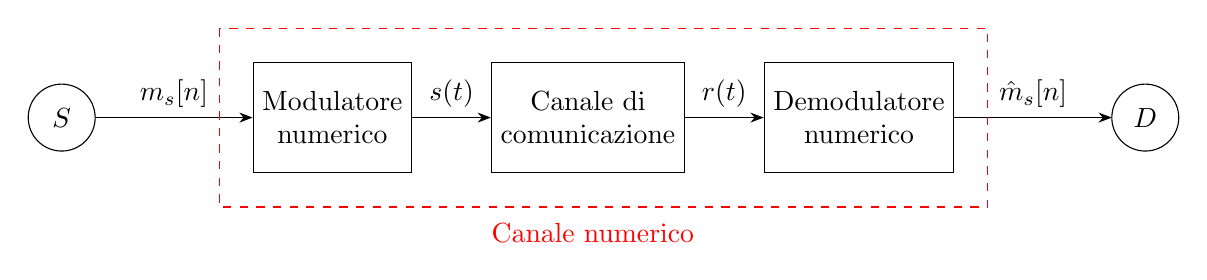
\begin{tikzpicture}[>=Stealth, block/.style={draw, rectangle}, scale=0.85]
            % Blocks
            \tikzstyle{block} = [rectangle, draw, text centered, minimum height=4em, align=center]

            \node[block] (mod) {Modulatore \\ numerico};
            \node[block, right=1cm of mod] (channel) {Canale di \\ comunicazione};
            \node[block, right=1cm of channel] (demod) {Demodulatore \\ numerico};

            % Nodes for connecting lines
            \coordinate[left=2cm of mod] (input);
            \coordinate[right=2cm of demod] (output);

            % Lines
            \draw[->] (input) -- node[above] {$m_s[n]$} (mod);
            \draw[->] (mod) -- node[above] {$s(t)$} (channel);
            \draw[->] (channel) -- node[above] {$r(t)$} (demod);
            \draw[->] (demod) -- node[above] {$\hat{m}_s[n]$} (output);

            % Dashed box
            \begin{scope}
                \draw[dashed, red] ($(mod.north west)+(-0.5,0.5)$) rectangle ($(demod.south east)+(0.5,-0.5)$);
            \end{scope}

            % Annotations
            \node[align=center, red, above right= -1cm and -6cm of demod.south east] (channel-label) {Canale numerico};

            % Circles
            \draw (input) ++(-0.5cm,0) circle (0.5cm) node {$S$};
            \draw (output) ++(0.5cm,0) circle (0.5cm) node {$D$};
        \end{tikzpicture}












\end{document}

    \end{center}
\end{adjustwidth*}


In una comunicazione digitale l'informazione è codificata in sequenze di bit. Se rappresentassimo ogni bit come un funzione delta otterremmo un treno di delta:
\[
    \sum_{k=-\infty}^{+\infty} d_k \delta(t - kT_b)
\]
che occupa però una banda infinita.

La modulazione PAM consiste nell'effettuare la mappatura dei bit ed effettuare un filtraggio con un filtro passa basso avente risposta all'impulso \( g_T(t) \), ottenendo:
\[ s_{PAM}(t) = \sum_{k=-\infty}^{+\infty} a_k\cdot g_T(t - kT_s) \]

Una sequenza di bit può essere trattata come una variabile aleatoria con distribuzione uniforme:
\[
    \mathbb{P}(d_k = 0) = \mathbb{P}(d_k = 1) = \frac{1}{2} 
\]
\[
    \mathbb{E}\{d_k\} = 0\cdot \mathbb{P}(d_k = 0) + 1\cdot \mathbb{P}(d_k = 1) = \frac{1}{2}
\]

\[
    E_{s_{PAM}}(i) = \int_{-\infty}^{+\infty} s_{PAM, i}^2(t) \, dt =  \int_{-\infty}^{+\infty} \alpha_i^2 \cdot g_T^2(t - kT_s) \, dt = \int_{-\infty}^{+\infty} (2i - 1 - M)^2 g_T^2(t) \, dt = (2i - 1 - M)^2 E_{g_T}
\]

Scegliendo una mappatura simmetrica dei bit, possiamo trasmettere simboli con media nulla e quindi con energia a media nulla:
\[
    a_i = 
    \begin{cases}
        -1 & \text{se } d_k = 0 \\
        1 & \text{se } d_k = 1
    \end{cases}
\]
Per \( M \) pari si ha \( A_s = \{ \pm 1, \pm 3, \ldots, \pm (M-1) \} \)

Per \( M \) dispari si ha \( A_s = \{ 0, \pm 2, \pm 4, \ldots, \pm (M-1) \} \)


Gli \( M \) valori \( (M \geq 2) \) che costituiscono l'alfabeto \( A_s = \{ \alpha_1, \alpha_2, \ldots, \alpha_M \} \) sono definiti come:
\[ \alpha_i = 2i - 1 - M, \quad i = 1, 2, \ldots, M \]




\subsection*{Proprietà derivate della M-PAM}
\begin{enumerate}
    \item Il valor medio di \( s(t) \) è zero per ogni \( t \):
          \begin{equation*}
              \mathbb{E}\left[ s(t) \right] = 0 \quad \forall t
          \end{equation*}
          \begin{equation*}
              \mathbb{E} \left[ \sum_{k=-\infty}^{+\infty} a[k] \ g_T(t-kT_s) \right] = \sum_{k=-\infty}^{+\infty} \mathbb{E}\left[a[k]\right]\ g_T(t-kT_s) = 0
          \end{equation*}
          \begin{equation*}
              \mathbb{E}\left[a[k]\right] = \frac{1}{M} \sum_{i=1}^{M} \alpha_i \mathbb{P}\{\alpha_i\} = \frac{1}{M} \sum_{i=1}^{M} (2i - 1 - M)
          \end{equation*}
          \begin{equation*}
              = \frac{2}{M} \sum_{i=1}^{M} i - 1 - M = \frac{2}{M} \frac{M(M+1)}{2} - (M+1) = 0
          \end{equation*}

    \item La densità spettrale di potenza invece è:
          \begin{equation*}
              S_s(f) = \frac{1}{T_s} S_a(f) \ |G_T(f)|^2
          \end{equation*}
          \begin{equation*}
              \text{dove } \sigma_a^2 = \mathbb{E}\left[ a\left[k\right]^2 \right] = \frac{(M-1)(M+1)}{3}
          \end{equation*}
\end{enumerate}

\[
    R_s(t,\tau) = \mathbb{E}[s(t) \ s^*(t-\tau)]
\]
\[
    = \mathbb{E} \left[ \sum_{n=-\infty}^{+\infty} a\left[n\right] g_T(t - nT_s) \sum_{k=-\infty}^{+\infty} a^*\left[k\right] g_T^*(t - \tau - kT_s) \right]
\]
\[
    = \sum_{n=-\infty}^{+\infty} \sum_{k=-\infty}^{+\infty} \mathbb{E}[a\left[n\right] a^*\left[k\right]] \cdot g_T(t - nT_s) \cdot g_T^*(t - \tau - kT_s)
\]
\[
    = \sum_{n=-\infty}^{+\infty} \sum_{k=-\infty}^{+\infty} R_a\left[n-k\right] \cdot g_T(t - nT_s) \cdot g_T^*(t - \tau - kT_s)
\]

Imponendo \( n-k = m \) abbiamo che \( k = n-m \), quindi:

\[
    = \sum_{m=-\infty}^{+\infty} R_a[m] \sum_{n=-\infty}^{+\infty} g_T(t - nT_s) \cdot g_T^*(t - \tau - nT_s + mT_s)
\]

\paragraph*{Autocorrelazione media}

La funzione di autocorrelazione media \( \overline{R}_s(\tau) \) è:
\begin{align*}
    \overline{R}_s(\tau) & = \lim_{T\to\infty} \frac{1}{T} \int_{-\frac{T}{2}}^{\frac{T}{2}} R_s(t, \tau) dt                                                                   \\
    \overline{R}_s(\tau) & = \frac{1}{T_0} \int_{-\frac{T_0}{2}}^{\frac{T_0}{2}} R_s(t,\tau)dt \quad \text{se} \quad R_s(t,\tau) \quad \text{è periodico in} t           \\
    \overline{R}_s(\tau) & = \sum_{m=-\infty}^{\infty} R_a[m] \frac{1}{T_s} \sum_{n=-\infty}^{\infty} \int_{-\frac{T_s}{2}}^{\frac{T_s}{2}} g_T(t-nT_s)g_T^*(t-\tau-nT_s+mT_s)dt   \\
                         & = \sum_{m=-\infty}^{\infty} R_a[m] \frac{1}{T_s} \sum_{n=-\infty}^{\infty}\int_{-\frac{T_s}{2}+nT_s}^{\frac{T_s}{2}+nT_s} g_T(t')g_T^*(t'-\tau+mT_s)dt' \\
                         & = \sum_{m=-\infty}^{\infty} R_a[m] \frac{1}{T_s} \int_{-\infty}^{\infty} g_T(t')g_T^*(t'-\tau+mT_s)dt'                                                  \\
                         & = \sum_{m=-\infty}^{\infty} R_a[m] \frac{1}{T_s} \int_{-\infty}^{\infty} G_T(f)[G_T(f)e^{-j2\pi f\tau}e^{j2\pi fmT_s}]^*df                              \\
                         & = \int_{-\infty}^{\infty} G_T(f)G_T^*(f)\frac{1}{T_s} \sum_{m=-\infty}^{\infty} R_a[m] e^{-j2\pi fmT_s}e^{j2\pi f\tau}df                                \\
                         & = \frac{1}{T_s} \int_{-\infty}^{\infty} |G_T(f)|^2 S_a(f)e^{j2\pi f\tau}df
\end{align*}


\[
    \overline{R}_s(\tau) = \frac{1}{T_s} TCF^{-1} \left[ |G_T(f)|^2 S_a(f) \right]
\]
\[
    \Rightarrow S_s(f) = \frac{1}{T_s} S_a(f) |G_T(f)|^2
\]

Nel caso in cui:
\begin{enumerate}
    \item $\mathbb{E} [ a_n ] = 0$
    \item $R_a[m] = \sigma_a^2 \delta[m]$
\end{enumerate}

Si ha che:
\[
    S_s(f) = \frac{\sigma_a^2}{T_s} |G_T(f)|^2
\]

In questo caso la $B_T$ coincide con quella del filtro $G_T(f)$.

Calcolo di $\sigma_a^2$:
\[
    \sigma_a^2 = \mathbb{E} \left[ (a - \mu_a)^2 \right] = \int_{-\infty}^{\infty} (a - \mu_a)^2 f_a(a) da
\]
\[
    = \frac{1}{M} \sum_{i=1}^{M} (2i - 1 - M)^2
\]
\[
    = \frac{1}{M} \left[ 4 \sum_{i=1}^{M} i^2 + (1+M)^2 M - 4(1+M) \sum_{i=1}^{M} i \right]
\]

Sfruttando i seguenti risultati noti:
\[
    \sum_{i=1}^{n} i^2 = \frac{n(n+1)(2n+1)}{6}, \quad \sum_{i=1}^{n} i = \frac{n(n+1)}{2}
\]

Si ottiene:
\[
    \sigma_a^2 = \frac{M^2 - 1}{3}
\]


\[
    P_s = \frac{\sigma_a^2 E_{g_T}}{T_s} = \frac{M^2 - 1}{3} \frac{E_{g_T}}{T_s}
\]


In banda passante invece si ha che:
\[
    \sigma_a^2 = \frac{M^2 - 1}{6}
\]
\[
    P_s = \frac{M^2 - 1}{6} \frac{E_{g_T}}{T_s}
\]

Come sarà dimostrato più avanti, $R_s \propto B$, dove $B$ è la banda del segnale $s_{PAM}(t)$. 
Per $R_s$ valgono le seguenti equivalenze:
\[
    R_s = \frac{1}{T_s} = \frac{1}{mT_s} = \frac{R_b}{m} = \frac{R_b}{\log_2 M}
\]

Dove $R_b$ è il bit rate.




\paragraph*{Efficienza Spettrale di una M-PAM}
\[
    \beta = \frac{R_b}{B_T} = \frac{\log_2 M}{T_s B_{g_T}}
\]
essendo \( B_T = B_{g_T} \),

L'efficienza spettrale aumenta con l'aumentare del numero di livelli. Sfortunatamente, come verrà dimostrato più avanti, l'efficienza in potenza diminuisce all'aumentare di \( M \).

\begin{center}
    \tikzsetnextfilename{pam_trasmitter}
    \documentclass{standalone}

\usepackage{tikz,pgf}
\usepackage[utf8]{inputenc}
\usepackage[colorlinks=true, allcolors=blue]{hyperref}
\usetikzlibrary{positioning, arrows.meta, fit, shapes}
\begin{document}


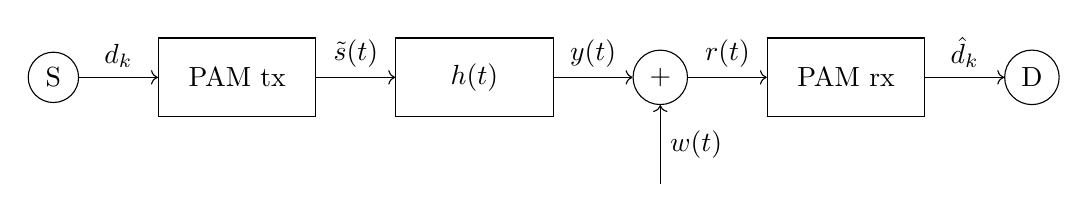
\begin{tikzpicture}[
            block/.style={rectangle, draw, minimum height=1cm, minimum width=2cm},
            node distance=1cm,
            auto
        ]
        \node[draw, circle] (source)  {S};
        \node[block, right= of source] (interpolatore) {PAM tx};
        \node[left=of interpolatore] (tmp) {};
        \node[block, right= of interpolatore] (chan) {$h(t)$};

        \node[draw, circle, right= of chan] (plus)  {\(+\)};
        \node[below=of plus, inner sep=0pt, minimum size=0pt] (n) {};
        \node[block, right=of plus] (sampler) {PAM rx};
        \node[circle, draw, right=of sampler] (dest) {D};
        
        \draw[->] (source) -- (interpolatore) node[midway,above] {$d_k$};
        \draw[->] (interpolatore) -- (chan) node[midway,above] {$\tilde{s}(t)$};
        \draw[->] (chan) -- (plus) node[midway,above] {$y(t)$};
        \draw[->] (plus) -- (sampler) node[midway,above] {$r(t)$};
        \draw[->] (n) -- (plus) node[midway, right] {$w(t)$};
        \draw[->] (sampler) -- (dest) node[midway,above] {$\hat{d}_k$};
    \end{tikzpicture}



\end{document}

\end{center}


Il canale di comunicazione è generalmente modellato come un sistema LTI, caratterizzato da una risposta impusliva $h(t)$ e da un rumore additivo $w(t)$.
Nel caso ideale $h(t) = \delta (t)$.
Il rumore aggiunto al segnale si modella come rumore bianco gaussiano a potenza spettrale costante $N_0/2$, col quale si modella il disturbo proveniente dalle radiazioni solari, dalle radiazioni del big bang e del rumore dei dispositivi.
Il ricevitore è composto da 3 componenti principali:
\begin{enumerate}
    \item \textbf{Filtro passa basso}, che filtra il segnale ricevuto per eliminare le frequenze superiori a $B_T$.
    \item \textbf{Campionatore}, che campiona il segnale filtrato con rate $1/T_s$. 
    \item \textbf{Decisore}, che associa ad ogni campione un simbolo appartenente alla costellazione.
\end{enumerate}
Il segnale ricevuto è il seguente:
\[
    r(t) = s(t) \ast h(t) + w(t)
\]

mentre il segnale filtrato è:
\[
    x(t) = r(t) \ast g_R(t) = \sum_{k=-\infty}^{+\infty} a_k g(t - kT_s) + n(t)
\]
dove $g(t) = g_T(t) \ast h(t) \ast g_R(t)$ e $n(t) = w(t) \ast g_R(t)$. La densità spettrale di energia del rumore diventa:
\[
    S_n(f) = S_w(f) |G_R(f)|^2
\]



\subsection*{Interferenza intersimbolica (ISI)}
\noindent
\begin{minipage}{.5\textwidth}
    \centering
    \textbf{Assenza di ISI:}
    \[
        x[k] = f(a[k])
    \]
    \\
\end{minipage}%
\begin{minipage}{.5\textwidth}
    \centering
    \textbf{Presenza di ISI:}
    \[
        x[k] = f(\dots, a[k-1], a[k], a[k+1], \dots)
    \]
    \\
\end{minipage}


Il risultato è che il campione estratto al ricevitore dal segnale ricevuto al $k$-esimo istante non dipende solo dal $k$-esimo simbolo.

\begin{center}
    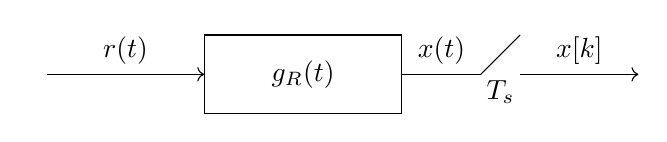
\begin{tikzpicture}[
            block/.style={rectangle, draw, minimum height=1cm, minimum width=2.5cm},
            node distance=1cm and 2cm,
            auto
        ]

        \node[block] (filter) {$g_R(t)$};
        \node[left=of filter] (channel) {};
        \node[right=of filter] (sampler) {};

        \draw[->] (channel) -- (filter) node[midway,above] {$r(t)$};

        \draw ([xshift=0]filter.east) -- ([xshift=1cm]filter.east) node[midway,above] {$x(t)$};
        \draw ([xshift=1cm]filter.east) -- ([xshift=1.5cm,yshift=0.5cm]filter.east) node[midway,below, yshift=-0.2cm] {$T_s$};

        \draw[->] ([xshift=1.5cm,yshift=0cm]filter.east) -- ++(1.5cm,0) node[midway,above] {$x[k]$};


    \end{tikzpicture}
\end{center}

dove:
\[
    x(t) = r(t) \ast g_R(t) = \sum_{k=-\infty}^{+\infty} a_k g(t - kT_s) + n(t)
\]
campionato in $t = mT_s$ si ha:
\[
        x(mT_s) = x[m] = \sum_{k=-\infty}^{+\infty} a_k g(mT_s - kT_s) + n(mT_s) = \sum_{k=-\infty}^{+\infty} a_k g[m-k] + n[m] \\ 
 \]
\[
        = a_m g(0) + \sum_{\substack{k \neq m,\\ k=-\infty}}^{+\infty} a_k g[m-k] + n[m]
\]



Un canale con banda \( B_c \) in generale introduce ISI. Ci sono due aspetti di cui ci occuperemo:

\begin{enumerate}
    \item Determinazione del \( T_s \) minimo che può essere adottato al fine di ottenere una sequenza campionata priva di ISI.
    \item Determinare le condizioni sotto le quali è possibile trasmettere un segnale M-PAM attraverso un canale non ideale in modo che non vi sia ISI nella sequenza campionata.
\end{enumerate}

Nel risolvere i due problemi riterremo \( h(t) \) fissata, e \( g_T(t) \) e \( g_R(t) \) variabili, in quanto determinabili dal progettista.

Un approccio non perseguibileconsiste nel trasmettere impulsi di durata finita e quindi con banda illimitata. Questo è in contrasto con la limitatezza messa a disposizione dal canale di trasmissione \( (B_c < \infty) \).

\(\Rightarrow\) Gli impulsi \( g_T(t) \) devono avere durata infinita.

\paragraph*{Criterio di Nyquist}{Primo criterio di Nyquist per la trasmissione priva di ISI}

\[ g(kT_s) =
    \begin{cases}
        1, & \text{se } k=0      \\
        0, & \text{se } k \neq 0
    \end{cases}
    \quad \text{(Dominio del tempo)}
\]

\[ \sum_{k=-\infty}^{+\infty} G\left(f-\frac{k}{T_s}\right) = T_s \quad \text{(Dominio della frequenza)} \]




\paragraph*{Dimostrazione}
Il criterio di Nyquist nel dominio del tempo garantisce l'assenza di ISI in quanto
\[ x[k] = a[k] \cdot g(0) + \sum_{\substack{i=-\infty \\ i \neq k}}^{+\infty} a[i] \cdot g[i-k] = a[k] \cdot g(0) \]
dove il secondo termine è nullo e non vi è ISI se \( g[k] = \delta[k] \).

La relazione in frequenza si ottiene come trasformazione
\[ g[k] = \delta[k] \quad \Longleftrightarrow \quad \overline{G}(f) = 1 \]
\[ \overline{G}(f) = \frac{1}{T_s} \sum_{k=-\infty}^{+\infty} G\left(f - \frac{k}{T_s}\right) = 1 \]
\[ \sum_{k=-\infty}^{+\infty} G\left(f - \frac{k}{T_s}\right) = T_s \]

\paragraph*{Trasmissione priva di ISI}
Supponiamo sia assegnato un canale a banda rigorosamente limitata con banda \( B_c \).
\[ H(f) = 0 \quad \text{per} \quad |f| > B_c \]
e supponiamo che \( B_T = B_c \), ovvero che il segnale trasmesso occupa tutta la banda messa a disposizione dal canale.
Allora si verificano le seguenti:
\begin{enumerate}
    \item Non è possibile in alcun modo eliminare l'ISI quando \( T_s < \frac{1}{2B_c} \).


          \paragraph*{Dimostrazione:}

          Quando \( T_s < \frac{1}{2B_c} \)

          \begin{tikzpicture}[scale=0.5]
              \draw[->] (-15,0) -- (15,0) node[right] {\( f \)};
              \draw[->] (0,-1) -- (0,7) node[above] {\( \overline{G}(f) \)};

              % Triangles
              \draw (-11,0) -- (-8,3) -- (-5,0);
              \draw[dashed, red] (-5,-1) -- (-5,4);
              \draw[dashed, red] (-3,-1) -- (-3,4);
              \draw (-3,0) -- (0,3) -- (3,0);
              \draw[dashed, red] (3,-1) -- (3,4);
              \draw[dashed, red] (5,-1) -- (5,4);
              \draw (5,0) -- (8,3) -- (11,0);

              \node at (-12,1.5) {\( \cdots \)};
              \node at (12,1.5) {\( \cdots \)};
          \end{tikzpicture}

          Esistono degli intervalli di frequenza dove \( \overline{H}(f) = 0 \) per cui non può mai accadere che \( \overline{H}(f) = 1 \) \( \forall f \)

          \bigskip

    \item Il più piccolo valore di \( T_s \) che permette di eliminare l'\( ISI \) è

          \( T_s^{(min)} = \frac{1}{2B_c} \)

          \bigskip

          \( f_s^{(max)}\) = \( \frac{1}{T_s^{(min)}} = 2B_c = f_N \) \quad (frequenza di Nyquist)

          \bigskip

          \begin{tikzpicture}[scale=0.5]
              \draw[->] (-15,0) -- (15,0) node[right] {\( f \)};
              \draw[->] (0,-1) -- (0,7) node[above] {\( \overline{G}(f) \)};

              % Triangles
              \draw (-9,0) -- (-6,3) -- (-3,0);
              \draw (-3,0) -- (0,3) -- (3,0);
              \draw (3,0) -- (6,3) -- (9,0);

              \node at (-10,1.5) {\( \cdots \)};
              \node at (10,1.5) {\( \cdots \)};
              \
          \end{tikzpicture}

          Non esistono intervalli di frequenza dove \( \overline{G}(f) = 0 \)

          \bigskip

    \item Nel caso valga la condizione \( T_s = \frac{1}{2B_c} \), allora l'unica funzione di trasferimento che permette di eliminare completamente l'ISI è

          \[ G(f) = \frac{1}{2B_c} \text{rect}\left(\frac{f}{2B_c}\right) \quad \Leftrightarrow \quad g(t) = \text{sinc}(2B_c t) \]

          \paragraph*{Dimostrazione:}

          \begin{center}

              \begin{tikzpicture}[scale=1]
                  \begin{axis}[
                          axis lines=middle,
                          xlabel={$f$},
                          ylabel={$G(f)$},
                          xtick={-4, -2, 2, 4},
                          xticklabels={$-2B_c$, $-B_c$, $B_c$, $2B_c$},
                          ytick={100},
                          yticklabels={},
                          ymin=-0.2, ymax=2,
                          xmin=-8, xmax=8,
                          xmajorgrids=false,
                          ymajorgrids=false,
                          clip=false
                      ]

                      \draw [thick] (axis cs:-2,0) rectangle (axis cs:2,0.4);

                      \node [red]at (axis cs:7,0.6) {$\sum_{k=-\infty}^{\infty} G(f - \frac{k}{T_s})$};

                      \draw [dashed, red] (axis cs:-6,0.4) -- (axis cs:-6,0);
                      \draw [dashed, red] (axis cs:-8,0.4) -- (axis cs:-2,0.4);
                      \draw [dashed, red] (axis cs:2,0.4) -- (axis cs:8,0.4);
                      \draw [dashed, red] (axis cs:6,0.4) -- (axis cs:6,0);
                  \end{axis}
                  \
              \end{tikzpicture}
          \end{center}

          Si nota anche che la funzione $\text{sinc}(2Bt)$ si annulla quando $t = \frac{k}{2B}$ con $k \neq 0$ per cui
          \[
              g(kT_s) = \text{sinc} \left(2B_c\cdot\frac{k}{2B_c}\right) = \text{sinc}(k) = 
              \begin{cases}
                  1 & \text{se } k=0    \\
                  0 & \text{se } k\neq0
              \end{cases}
          \]
\end{enumerate}


\textbf{Limiti di applicabilità della funzione di trasferimento rettangolare:}

\begin{enumerate}
    \item Realizzabilità di una funzione di trasferimento rettangolare: risposte in frequenza ideali come quella rettangolare non sono fisicamente realizzabili (Criterio di Paley-Wiener).
    \item Piccoli errori di campionamento provocano un ISI molto grande poiché la funzione $\text{sinc}(2B_ct)$ decresce molto lentamente.
\end{enumerate}

Un errore nel campionatore induce un ISI grande in quanto si sommano molte contributi!




\begin{figure}[ht]
    \centering
    \begin{center}
        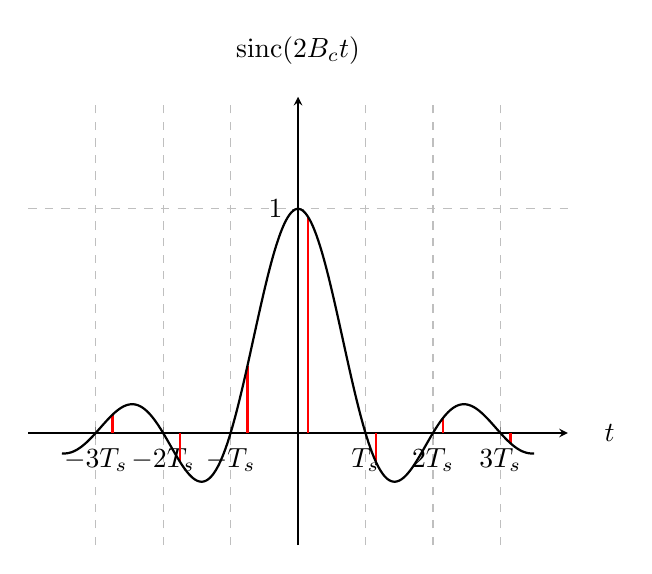
\begin{tikzpicture}
            \begin{axis}[
                    axis lines=middle,
                    xlabel={$t$},
                    ylabel={$\text{sinc}(2B_c t)$},
                    xtick={-3, -2, -1, 0, 1, 2, 3},
                    xticklabels={$-3T_s$, $-2T_s$, $-T_s$, $0$, $T_s$, $2T_s$, $3T_s$},
                    ytick={1},
                    ymin=-0.5, ymax=1.5,
                    xmin=-4, xmax=4,
                    every axis x label/.style={at={(ticklabel* cs:1.05)}, anchor=west,},
                    every axis y label/.style={at={(ticklabel* cs:1.05)}, anchor=south,},
                    xmajorgrids=true,
                    ymajorgrids=true,
                    grid style=dashed,
                    clip=false,
                    no markers,
                    samples=1000,
                    domain=-3.5:3.5
                ]


                \draw [thick, red] (axis cs:-2.75,0) -- (axis cs:-2.75,0.082);
                \draw [thick, red] (axis cs:-1.75,0) -- (axis cs:-1.75,-0.13);
                \draw [thick, red] (axis cs:-0.75,0) -- (axis cs:-0.75,0.30);

                \draw [thick, red] (axis cs:0.15,0) -- (axis cs:0.15,0.965);

                \draw [thick, red] (axis cs:1.15,0) -- (axis cs:1.15,-0.125);
                \draw [thick, red] (axis cs:2.15,0) -- (axis cs:2.15,0.07);
                \draw [thick, red] (axis cs:3.15,0) -- (axis cs:3.15,-0.045);


                % Define sinc function
                \addplot+[thick, black, smooth, unbounded coords=jump] {sin(deg(pi*x))/(pi*x)};
                \addplot+[thick, black, smooth] coordinates {(0, 1)};

                % Add the red vertical line at t=0

            \end{axis}
        \end{tikzpicture}
    \end{center}
    \caption*{Un errore $\epsilon$ nel campionatore induce un ISI grande in quanto si sommano molti contributi. In rosso l'errore $\epsilon$ del compionatore.}
    %\label{fig:my_label} % Optional, for referencing the figure
\end{figure}



Rilassando la condizione $T_s > \frac{1}{2B_c}$, ovvero ammettendo

\[ T_s > \frac{1}{2B_c} \]

si ottiene il seguente effetto:

\begin{center}

    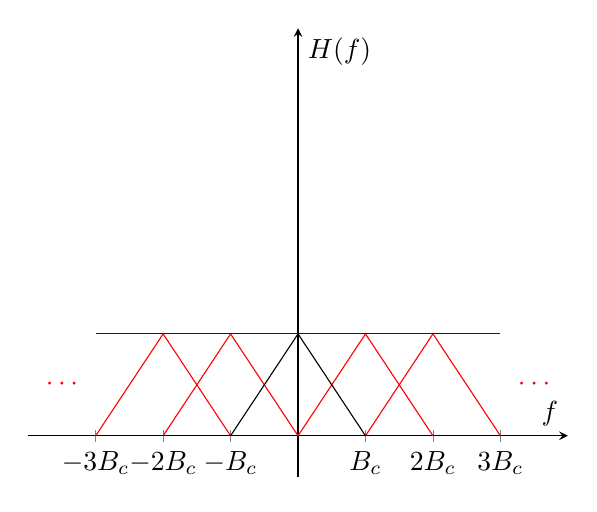
\begin{tikzpicture}[scale=1]
        \begin{axis}[
                axis lines=middle,
                xlabel={$f$},
                ylabel={$H(f)$},
                xtick={-6, -4, -2, 2, 4, 6},
                xticklabels={$-3B_c$, $-2B_c$, $-B_c$, $B_c$, $2B_c$, $3B_c$},
                ytick={100},
                yticklabels={},
                ymin=-0.2, ymax=2,
                xmin=-8, xmax=8,
                %every axis x label/.style={at={(ticklabel* cs:1.05)}, anchor=west,},
                %every axis y label/.style={at={(ticklabel* cs:1.05)}, anchor=south,},
                xmajorgrids=false,
                ymajorgrids=false,
                clip=false
            ]

            \node[red] at (-7,0.25) {\( \cdots \)};

            \draw[red] (-6,0) -- (-4,0.5) -- (-2,0);
            \draw[red] (-4,0) -- (-2,0.5) -- (0,0);

            \draw[red] (0,0) -- (2,0.5) -- (4,0);
            \draw[red] (2,0) -- (4,0.5) -- (6,0);

            \node[red] at (7,0.25) {\( \cdots \)};

            \draw[blue] (-6,0.5) -- (6,0.5);

            \draw (-2,0) -- (0,0.5) -- (2,0);


        \end{axis}
    \end{tikzpicture}
\end{center}

La sovrapposizione permette di definire una classe di infinite funzioni di trasferimento che soddisfano il primo criterio di Nyquist.

In questo caso però $B_c > \frac{1}{2T_s}$, per cui al punto di $T_s$ c'è bisogno di una banda disponibile nel canale che è maggiore di quella che occorre con la funzione di trasferimento rettangolare.

\subsection*{Filtro a coseno rialzato}

% Define the piecewise function
\[ H_{rc}(f) =
    \begin{cases}
        T_s                                                                                                          & \text{if } 0 \leq |f| \leq \frac{1-\alpha}{2T_s}                  \\
        \frac{T_s}{2} \left[ 1 - \sin\left(\frac{\pi T_s}{\alpha} \left( |f| - \frac{1}{2T_s} \right)\right) \right] & \text{if } \frac{1-\alpha}{2T_s} < |f| \leq \frac{1+\alpha}{2T_s} \\
        0                                                                                                            & \text{if } |f| > \frac{1+\alpha}{2T_s}
    \end{cases}
\]

con $0 < \alpha < 1$.

\begin{center}

    \definecolor{myblue}{RGB}{30,144,255}
    \definecolor{myred}{RGB}{178,34,34}
    \begin{tikzpicture}
        \begin{axis}[
                axis lines=middle,
                xlabel={$f$},
                ylabel={$H_{RC}(f)$},
                xtick={-0.5, 0.5},
                xticklabels={$\frac{-1}{2T_s}$, $\frac{1}{2T_s}$},
                ytick={0.5},
                yticklabels={$T_s/2$},
                ymin=0, ymax=1.5,
                xmin=-1, xmax=1,
                every axis x label/.style={at={(ticklabel* cs:1.05)}, anchor=west,},
                every axis y label/.style={at={(ticklabel* cs:1.05)}, anchor=south,},
                xmajorgrids=false,
                ymajorgrids=false,
                clip=false,
                no markers,
            ]

            % Draw the ideal filter response (black box)
            \draw [thick] (axis cs:-0.5,0) -- (axis cs:-0.5,1) -- (axis cs:0.5,1) -- (axis cs:0.5,0);

            % Draw the realistic filter response for alpha = 0.5 (blue line)
            % \addplot [myblue, thick, smooth, domain=-1:1] {0.5+0.5*cos(deg(pi*x))};
            \addplot [myblue, thick, smooth, domain=-0.75:0.-0.25] {0.5 * (1 + cos(deg(pi*(abs(x)-0.25)/0.5)))};
            \addplot [myblue, thick, smooth, domain=0.25:0.75] {0.5 * (1 + cos(deg(pi*(abs(x)-0.25)/0.5)))};


            % Draw the realistic filter response for alpha = 1 (red dashed line)
            \addplot [myred, thick, dashed, smooth, domain=-1:1] {0.5-0.5*sin(deg(pi*(abs(x)-0.5))};

            % Add annotations for alpha values
            \node[myblue] at (axis cs:0.75,0.8) {$\alpha=0.5$};
            \node at (axis cs:-0.75,0.8) {$\alpha=0$};
            \node[myred] at (axis cs:0.9,0.2) {$\alpha=1$};

            % Add black dot at intersection
            \node[circle,fill,inner sep=1.5pt] at (axis cs:0,0.5) {};

        \end{axis}
    \end{tikzpicture}
\end{center}
\subsection*{Propriet\`a}
\begin{enumerate}
    \item Quando \( \alpha = 0 \) il coseno rialzato coincide con la funzione di trasferimento rettangolare
    \item La banda \( B_H \) \`e direttamente ottenibile da \( B_H = \frac{1+\alpha}{2T_S} \)
\end{enumerate}

La \( h_{RC}(t) \) \`e calcolabile in forma chiusa:

\[ h_{RC}(t) = \sin\left(\frac{t}{T_S}\right) \frac{\cos\left(\frac{\alpha \pi t}{T_S}\right)}{\left(1- \frac{2\alpha t}{T_S}\right)^2}  \]

\[ h_{RC}(kT_S) = \delta[k] \]

\begin{itemize}
    \item Soddisfa il criterio di Nyquist nel tempo, per cui garantisce l'assenza di ISI
    \item Decresce per \( t \rightarrow \infty \) come \( \frac{1}{|t|^3} \) per \( \alpha > 0 \) quindi molto pi\`u velocemente del caso \( \alpha = 0 \) (rettangolare)
\end{itemize}


\paragraph*{Rumore}
Nel caso della banda passante il rumore dell'inviluppo complesso è definito come:
\[
    w(t) = w_I(t) + jw_Q(t) 
\]
e la densità spettrale di potenza è:
\[
    S_w(f) = 2N_0
\]


Dove sia la parte reale che immaginaria danno un contributo $N_0$. Il segnale originale presentava invece un rumore con densità spettrale di potenza $N_0/2$.
Dopo il filtraggio la densià spettrale di potenza del rumore assume la forma:
\[
    S_n(f) = S_w |G_R(f)|^2 = 2N_0 |G_R(f)|^2
\]

Il ricevitore deve quindi essere implementato al fine di minimizzare l'effetto del rumore, ovvero massimizzare l'SNR.

\paragraph*{Filtro adattato}
La massimizzazione dell'SNR si ottiene con un filtro adattato, dove:
\[
    g_R(t) = g_T(-t) \quad \Longleftrightarrow \quad G_R(f) = G_T^*(f)
\]

Volendo quindi soddisfare il criterio di Nyquist col coseno rialzato e volendo utilizzare il filtro adattato, otteniamo:
\[
    G(f) = G_T(f) H(f) G_R(f) = |G_T(f)|^2 H(f)
\]

Nel caso di canale ideale, definendo come $H_{SRRC} = \sqrt{H_{RC}}$ si ottiene:
\[
    g_T(t) = h_{SRRC}(t) \quad \Longleftrightarrow \quad G_T(f) = H_{SRRC}(f) 
\]

\[
    g_R(t) = h_{SRRC}(-t) \quad \Longleftrightarrow \quad H_R(f) = H_{SRRC}^*(f)
\]


In tal caso e considerando i simboli a media nulla ed equiprobabli: 
\[
    S_s(f) = \frac{1}{T_s} S_a |G_T(f)|^2 = \frac{A}{T_s} H_{RC}(f)
\]


Per quanto riguarda la banda invece:
\[
    B^{(BB)} = \frac{1+\alpha}{2T_s} = \frac{1+\alpha}{2} \frac{1}{\log_2(M) T_b} = \frac{1+\alpha}{2} \frac{R_b}{\log_2(M)} \quad \text{banda inviluppo complesso PAM}
\]
\[
    B^{(PB)} = 2 B^{(BB)} = (1+\alpha) \frac{R_b}{\log_2(M)} \quad \text{banda PAM in banda passante}
\]

\[
    P_s^{(BB)} = \int_{-\infty}^{+\infty} S_s(f) df = \frac{A}{T_s} \int_{-\infty}^{+\infty} H_{RC}(f) df = \frac{A}{T_s} h_{RC}(0) = \frac{A}{T_s} \quad \text{potenza media inviluppo complesso}
\]

\[
    P_s^{(PB)} = \frac{1}{2} P_s^{(BB)} = \frac{A}{2T_s} \quad \text{potenza media PAM in banda passante}
\]

\[
    E_s = P_s T_s = \frac{A}{2} = \frac{M^2 - 1}{6} \quad \text{energia media per simbolo}
\]


\section*{Strategia di decisione}


\[
    x[m] = a_m + n[m] = a_m + n_I[m] + jn_Q[m]
\]  

La potenza del segnale di disturbo può essere calcolatora considerando la densità spettrale di potenza:
\[
    P_n = \int_{-\infty}^{+\infty} S_n(f) df = 2N_0 \int_{-\infty}^{+\infty} |G_R(f)|^2 df = 2N_0 \int_{-\infty}^{+\infty} |H_{RC}(f)|^2 df = 2N_0
\]

Essendo il rumore a media nulla, la varianza del rumore è pari alla sua potenza:
\[
    \sigma_n^2 = P_n = 2N_0
\]

Quindi la variabile aleatoria associata al rumore ha distribuzione del tipo $\mathcal{N}(0, 2 N_0)$.

Si può dimostrare che in presenza di filtro RRC e simboli equiprobabili la strategia di dicisione ottima consiste nel massimizzare la probabilità condizionata di aver ricevuto $a^{(i)}$ sapendo di aver ricevuto $x[m]$:

\[
    \hat{a}_m = \underset{i=1,\ldots,M}{\mathrm{argmax}} \ \mathbb{P}(a^{(i)}|x[m])
\]

Usando il criterio di massima verosimiglianza e la formula di Bayes di può dimostrare che:
\[
    \mathbb{P}(a^{(i)} \ | \ x[m]) \propto  \mathbb{P}(x[m] \ | \ a^{(i)})
\]

\[
    x[m] \ | \ a^{(i)}  = a^{(i)} + n[m] \quad \Rightarrow \quad x[m] \ | \ a^{(i)} \sim \mathcal{N}(a^{(i)}, \sigma_n^2)
\]

\[
    f_X(x \ | \ a^{(i)}) = f_{W}(x - a^{(i)}) = \frac{1}{\sqrt{2\pi \sigma_n^2}} e^{-\frac{(x - a^{(i)})^2}{2\sigma_n^2}}
\]


Essendo i simboli reali e quindi anche il segnale PAM, è possibile ignorare la componente in quadratura del segnale ricevuto, in quanto non vi sarà alcuna informazione.
\[
    x[m] \ | \ a^{(i)} \sim \mathcal{N}(a^{(i)}, N_0) \quad \Rightarrow \quad f_X(x \ | \ a^{(i)}) = \frac{1}{\sqrt{2\pi \sigma_n^2}} e^{-\frac{(x - a^{(i)})^2}{2\sigma_n^2}}
\]
Il massimo della densità di probabilità è ottenuto minimizzando l'opposto dell'esponente:
\[
    \hat{a}_m = \underset{i=1,\ldots,M}{\mathrm{argmin}} \left| x[m] - a^{(i)} \right| 
\]

Per adottare il criterio di decisione ottimo si possono definire regioni non sovrapposte, all'interno delle quali il segnale ricevuto è associato a un determinato simbolo.
Ogni regione è composta da due punti il cui simbolo più vicino è $a^{(i)}$, nel caso di più simboli le due regioni agli estremi avranno una larghezza infinita, mentre quelle interne saranno limitate.
Le soglie sono date dal punto medio tra i due simboli adiacenti:
\[
    Z^{(i)} = \left\{ x \mid d(x, a^{(i)}) < d(x, a^{(j)}), j \neq i, j = 1, \ldots, M \right\}
\]

% include image in img/regions.jpg
%\begin{figure}[ht]
%    \centering
%    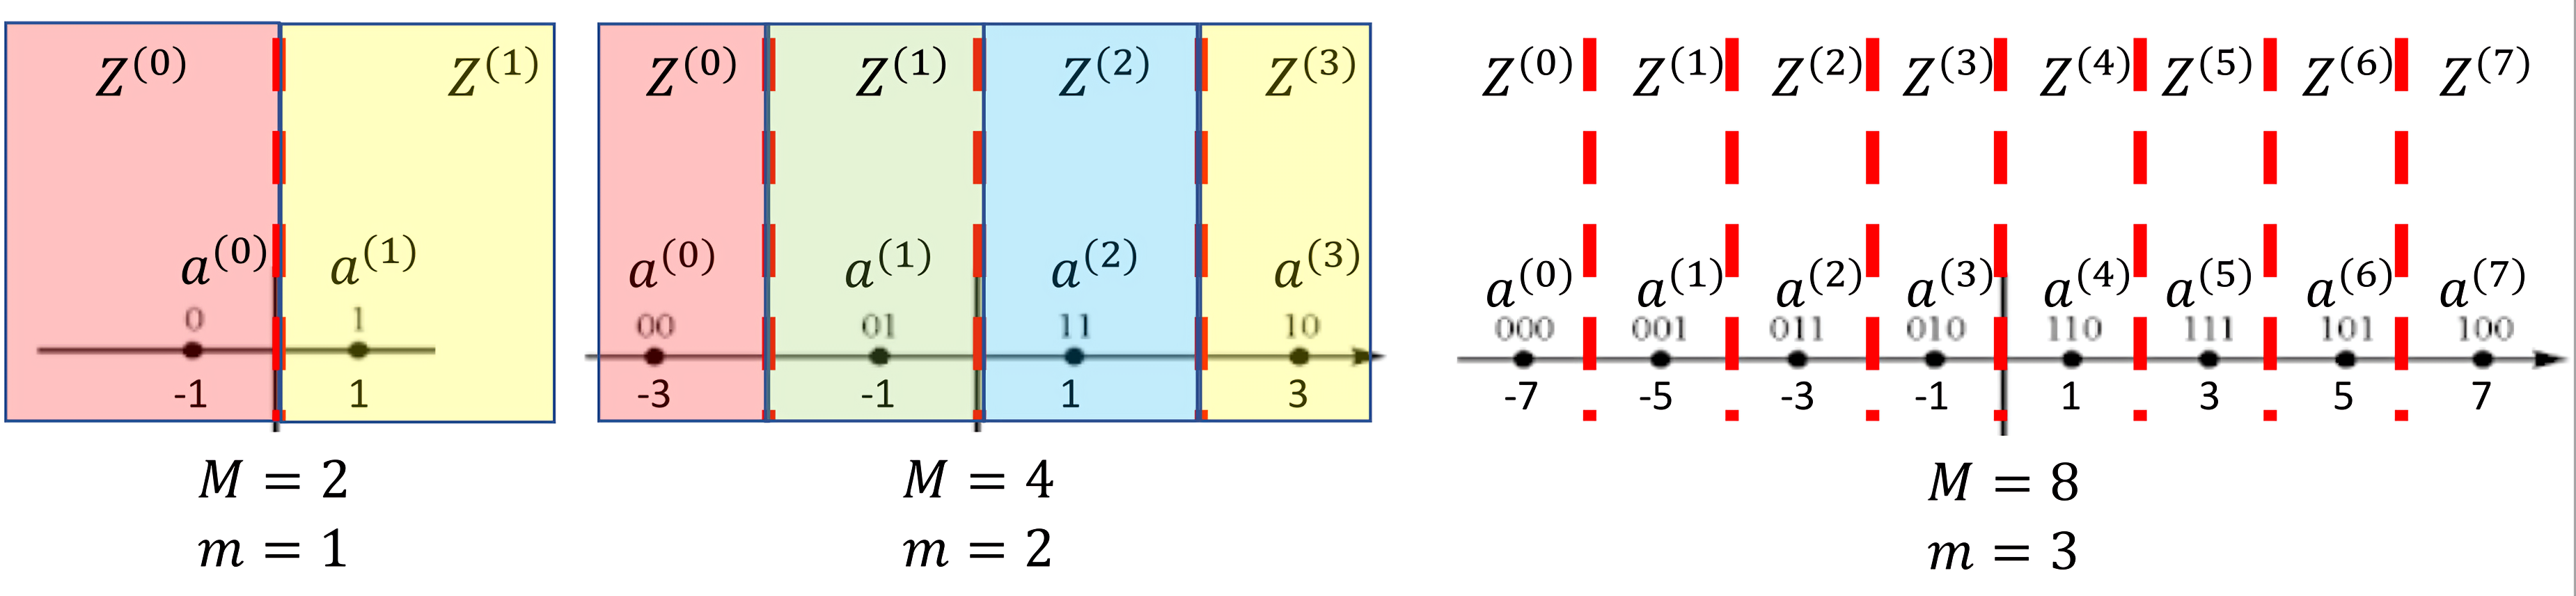
\includegraphics[width=0.875\textwidth]{imgs/regions.png}
%    \caption*{Regioni di decisione per un sistema PAM}
%\end{figure}

\begin{center}
    \tikzsetnextfilename{2PAM_decisor}
    \documentclass{standalone}
\usepackage{tikz}
\usetikzlibrary{positioning, decorations.pathreplacing}

\begin{document}
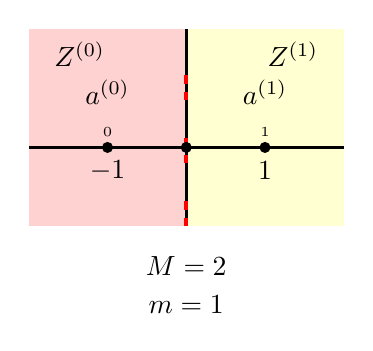
\begin{tikzpicture}

% Define colors
\definecolor{myred}{RGB}{255, 210, 210}
\definecolor{myyellow}{RGB}{255, 255, 210}

% Draw the rectangles
\fill[myred] (-2, 0) rectangle (0, 2.5);
\fill[myyellow] (0, 0) rectangle (2, 2.5);

% Vertical line in the middle
\draw[very thick] (0, 0) -- (0, 2.5);
% Draw the dashed lines in red
\draw[red, ultra thick, dashed] (0, 0) -- (0, 0.4);
\draw[red, ultra thick, dashed] (0, 0.8) -- (0, 1.2);
\draw[red, ultra thick, dashed] (0, 1.6) -- (0, 2);

% Draw the horizontal line
\draw[thick] (-2, 1) -- (2, 1);

% Draw the nodes
\fill (0, 1) circle (2pt);
\fill (-1, 1) circle (2pt);
\fill (1, 1) circle (2pt);

% Add labels
\node at (-1, 1.2) {\textnormal{\tiny $0$}};
\node at (1, 1.2) {\textnormal{\tiny $1$}};

\node at (-1, 0.7) {$-1$};
\node at (1, 0.7) {$1$};

\node at (-1, 1.7) {$a^{(0)}$};
\node at (1, 1.7) {$a^{(1)}$};

\node[above right] at (-1.8, 1.9) {$Z^{(0)}$};
\node[above left] at (1.8, 1.9) {$Z^{(1)}$};

% Add the bottom text
\node at (0, -0.5) {$M=2$};
\node at (0, -1) {$m=1$};

\end{tikzpicture}
\end{document}



\end{center}

\begin{center}
    \tikzsetnextfilename{4PAM_decisor}
    \documentclass{standalone}
\usepackage{tikz}
\usetikzlibrary{positioning, decorations.pathreplacing}

\begin{document}
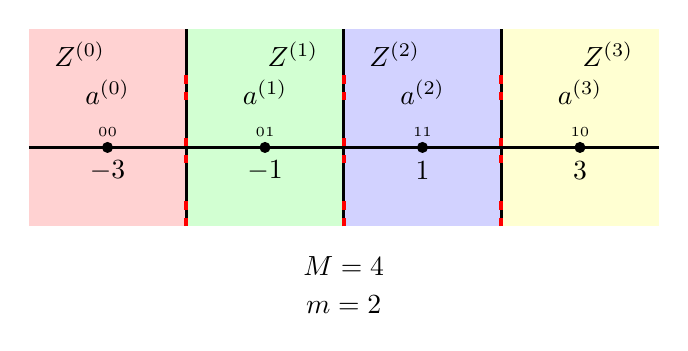
\begin{tikzpicture}

% Define colors
\definecolor{myred}{RGB}{255, 210, 210}
\definecolor{mygreen}{RGB}{210, 255, 210}
\definecolor{myblue}{RGB}{210, 210, 255}
\definecolor{myyellow}{RGB}{255, 255, 210}

% Draw the rectangles
\fill[myred] (-4, 0) rectangle (-2, 2.5);
\fill[mygreen] (-2, 0) rectangle (0, 2.5);
\fill[myblue] (0, 0) rectangle (2, 2.5);
\fill[myyellow] (2, 0) rectangle (4, 2.5);

% Vertical lines in the middle
\draw[very thick] (-2, 0) -- (-2, 2.5);
\draw[very thick] (0, 0) -- (0, 2.5);
\draw[very thick] (2, 0) -- (2, 2.5);

% Draw the dashed lines in red
\draw[red, ultra thick, dashed] (-2, 0) -- (-2, 0.4);
\draw[red, ultra thick, dashed] (-2, 0.8) -- (-2, 1.2);
\draw[red, ultra thick, dashed] (-2, 1.6) -- (-2, 2);

\draw[red, ultra thick, dashed] (0, 0) -- (0, 0.4);
\draw[red, ultra thick, dashed] (0, 0.8) -- (0, 1.2);
\draw[red, ultra thick, dashed] (0, 1.6) -- (0, 2);

\draw[red, ultra thick, dashed] (2, 0) -- (2, 0.4);
\draw[red, ultra thick, dashed] (2, 0.8) -- (2, 1.2);
\draw[red, ultra thick, dashed] (2, 1.6) -- (2, 2);

% Draw the horizontal line
\draw[thick] (-4, 1) -- (4, 1);

% Draw the nodes
\fill (-3, 1) circle (2pt);
\fill (-1, 1) circle (2pt);
\fill (1, 1) circle (2pt);
\fill (3, 1) circle (2pt);

% Add labels
\node at (-3, 1.2) {\textnormal{\tiny $00$}};`'
\node at (-1, 1.2) {\textnormal{\tiny $01$}};
\node at (1, 1.2) {\textnormal{\tiny $11$}};
\node at (3, 1.2) {\textnormal{\tiny $10$}};

\node at (-3, 0.7) {$-3$};
\node at (-1, 0.7) {$-1$};
\node at (1, 0.7) {$1$};
\node at (3, 0.7) {$3$};

\node at (-3, 1.7) {$a^{(0)}$};
\node at (-1, 1.7) {$a^{(1)}$};
\node at (1, 1.7) {$a^{(2)}$};
\node at (3, 1.7) {$a^{(3)}$};

\node[above right] at (-3.8, 1.9) {$Z^{(0)}$};
\node[above left] at (-0.2, 1.9) {$Z^{(1)}$};
\node[above right] at (0.2, 1.9) {$Z^{(2)}$};
\node[above left] at (3.8, 1.9) {$Z^{(3)}$};

% Add the bottom text
\node at (0, -0.5) {$M=4$};
\node at (0, -1) {$m=2$};

\end{tikzpicture}
\end{document}



\end{center}

\begin{center}
    \tikzsetnextfilename{8PAM_decisor}
    \documentclass{standalone}
\usepackage{tikz}
\usetikzlibrary{positioning, decorations.pathreplacing}

\begin{document}
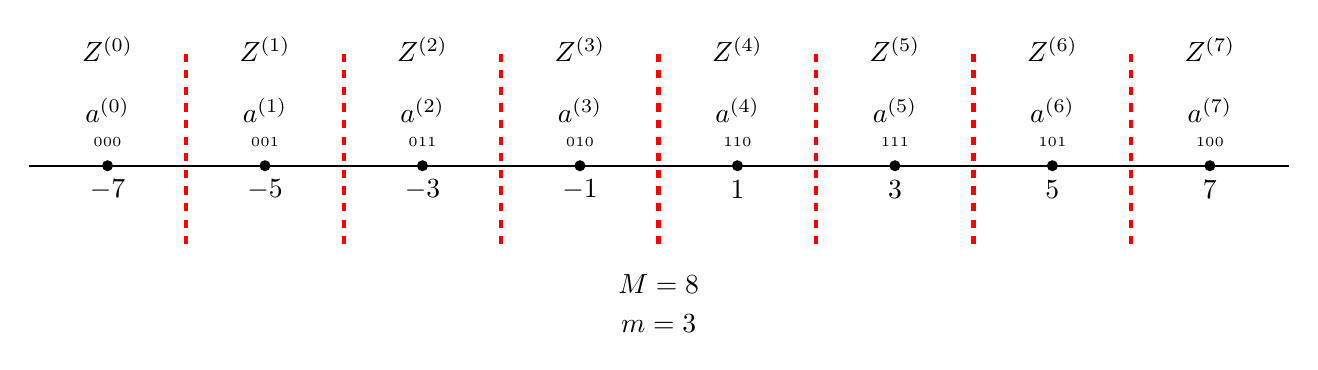
\begin{tikzpicture}

% Define colors
\definecolor{myred}{RGB}{255, 0, 0}

% Draw the horizontal line
\draw[thick] (-8, 1) -- (8, 1);

% Draw the nodes
\fill (-7, 1) circle (2pt);
\fill (-5, 1) circle (2pt);
\fill (-3, 1) circle (2pt);
\fill (-1, 1) circle (2pt);
\fill (1, 1) circle (2pt);
\fill (3, 1) circle (2pt);
\fill (5, 1) circle (2pt);
\fill (7, 1) circle (2pt);

% Add labels for a
\node at (-7, 0.7) {$-7$};
\node at (-5, 0.7) {$-5$};
\node at (-3, 0.7) {$-3$};
\node at (-1, 0.7) {$-1$};
\node at (1, 0.7) {$1$};
\node at (3, 0.7) {$3$};
\node at (5, 0.7) {$5$};
\node at (7, 0.7) {$7$};

% Add binary labels for a
\node at (-7, 1.3) {\textnormal{\tiny $000$}};
\node at (-5, 1.3) {\textnormal{\tiny $001$}};
\node at (-3, 1.3) {\textnormal{\tiny $011$}};
\node at (-1, 1.3) {\textnormal{\tiny $010$}};
\node at (1, 1.3) {\textnormal{\tiny $110$}};
\node at (3, 1.3) {\textnormal{\tiny $111$}};
\node at (5, 1.3) {\textnormal{\tiny $101$}};
\node at (7, 1.3) {\textnormal{\tiny $100$}};

% Add labels for a^(i)
\node at (-7, 1.7) {$a^{(0)}$};
\node at (-5, 1.7) {$a^{(1)}$};
\node at (-3, 1.7) {$a^{(2)}$};
\node at (-1, 1.7) {$a^{(3)}$};
\node at (1, 1.7) {$a^{(4)}$};
\node at (3, 1.7) {$a^{(5)}$};
\node at (5, 1.7) {$a^{(6)}$};
\node at (7, 1.7) {$a^{(7)}$};

% Draw the dashed lines in green
\draw[myred, ultra thick, dashed] (-6, 0) -- (-6, 2.5);
\draw[myred, ultra thick, dashed] (-4, 0) -- (-4, 2.5);
\draw[myred, ultra thick, dashed] (-2, 0) -- (-2, 2.5);
\draw[myred, ultra thick, dashed] (0, 0) -- (0, 2.5);
\draw[myred, ultra thick, dashed] (2, 0) -- (2, 2.5);
\draw[myred, ultra thick, dashed] (4, 0) -- (4, 2.5);
\draw[myred, ultra thick, dashed] (6, 0) -- (6, 2.5);

% Add labels for Z
\node[above] at (-7, 2.2) {$Z^{(0)}$};
\node[above] at (-5, 2.2) {$Z^{(1)}$};
\node[above] at (-3, 2.2) {$Z^{(2)}$};
\node[above] at (-1, 2.2) {$Z^{(3)}$};
\node[above] at (1, 2.2) {$Z^{(4)}$};
\node[above] at (3, 2.2) {$Z^{(5)}$};
\node[above] at (5, 2.2) {$Z^{(6)}$};
\node[above] at (7, 2.2) {$Z^{(7)}$};

% Add the bottom text
\node at (0, -0.5) {$M=8$};
\node at (0, -1) {$m=3$};

\end{tikzpicture}
\end{document}



\end{center}



Sebbene si adotti il criterio di decisione ottimo, la presenza del rumore può portare a una decisione errata, traslando il segnale in una regione non associata al simbolo trasmesso.
La probabilità di errore sul simbolo equivale alla probabilità di sovrastimare $a^{(i)}$ e il campione ricevuto non rientri nella regione $Z^{(i)}$:
\[
    P_e = \frac{1}{M} \sum_{i=0}^{M-1} \mathbb{P}(\text{errore} \ | \ a^{(i)}) = \lim_{N^{(s)} \to +\infty} \frac{N_e^{(s)}}{N^{(s)}} \quad \text{probabilità errore PAM}
\]

Considerando una modulazione 2-PAM, il campione ricevuto in presenza di rumore avrà una distribuzione gaussiana centrata in $a^{(i)}$, ovvero in $\pm 1$. Poiché la soglia è data da 0, nel caso sia stato trasmesso +1 (-1) la probabilità di errore corrisponde all'area della gaussiana a sinistra (destra) della soglia, centrata in 1 (-1).

% include imgs/2pamerror.jpg
\begin{figure}[ht]
    \centering
    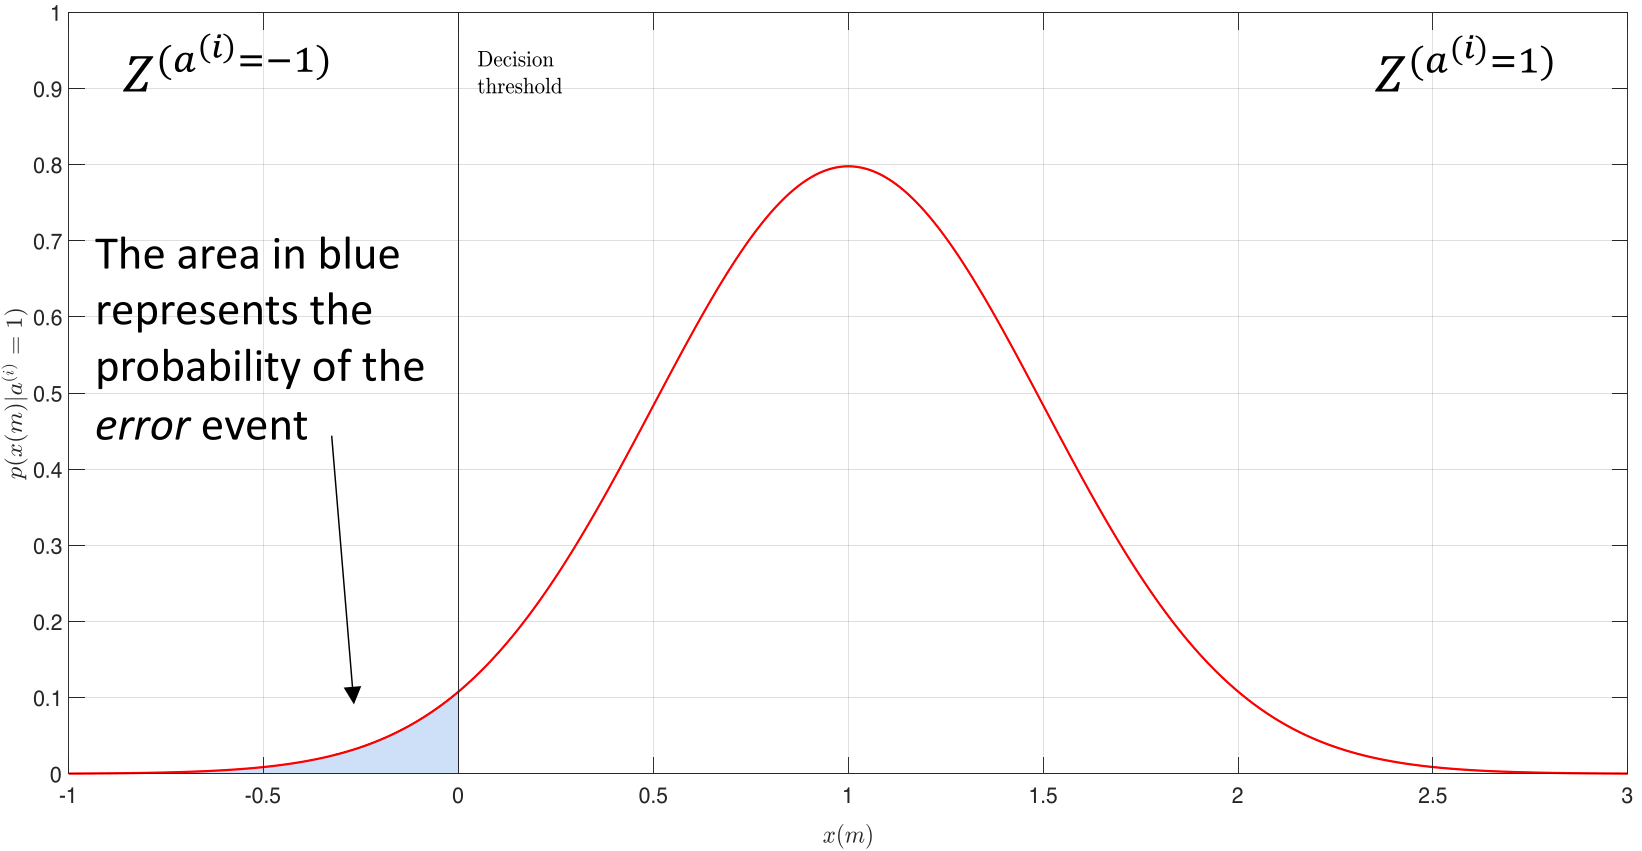
\includegraphics[width=0.65\textwidth]{imgs/2pamerror.jpg}
    \caption*{Probabilità di errore per una modulazione 2-PAM}
\end{figure}


Quindi la probabilità di errore in questo caso può essere espressa come:
\[
    P(e | -1) = Q\left(\frac{\text{d}(t_i, m_x)}{\sigma}\right) = Q\left(\frac{1}{\sigma}\right)
\]

Dove l'ultima uguaglianza deriva dal fatto che la soglia $t_i=0$ e il valore medio della gaussiana è $m_x = -1$.

Si ottiene il solito valore anche calcolando la probabilità di errore per il simbolo $+1$, quindi la probabilità di errore della 2-PAM equivale a:
\[
    P^{\text{2-PAM}}_e = \frac{1}{2} Q\left(\frac{1}{\sigma}\right) + \frac{1}{2} Q\left(\frac{1}{\sigma}\right) = Q\left(\frac{1}{\sigma}\right)
\]

Se i simboli scelti fossero stati $a^{(i)} = \{-3, -1, 1, 3\}$, la distanza tra simbolo e soglia sarebbe stata in ogni caso 1.
Per una 4-PAM la probabilità di errore è:

\[ 
    P^{\text{4-PAM}}_e = \frac{1}{4} \sum_{i=1}^{4} \mathbb{P}(e \mid a^{(i)}) = \frac{1}{4} \cdot 2 \left[ \mathbb{P}(e \mid a^{(i)} = 1) + \mathbb{P}(e \mid a^{(i)} = 3) \right] = \frac{1}{2} \left[ 2 Q\left( \frac{1}{\sigma} \right) + Q\left( \frac{1}{\sigma} \right) \right] = \frac{3}{2} Q\left( \frac{1}{\sigma} \right)
\]

Considerando che per la banda passante $E_s = \frac{M^2 - 1}{6}$, possiamo trovare la relazione:
\[
    1 = \frac{6 E_s}{(M^2 - 1)}
\]
Mentre ricordando che la varianza del rumore è $\sigma_n^2 = N_0$, possiamo esprimere la probabilità di errore in funzione della SNR ($\frac{E_s}{N_0}$):

\[
    P_e^{\text{M-PAM}} = \frac{2(M - 1)}{M} Q\left(\sqrt{\frac{6 E_s}{(M^2 - 1) N_0}}\right)
\]


Esprimendo i risultati in funzione della SNR ($\frac{E_s}{N_0}$), si ottiene:
\[
    \text{2-PAM:} \quad E_s = \frac{1}{2}, P^{\text{2-PAM}}_e = Q\left( \sqrt{\frac{2 E_s}{N_0}} \right)
\]
\[
    \text{4-PAM:} \quad E_s = \frac{5}{2}, P^{\text{4-PAM}}_e = \frac{3}{2} Q\left( \sqrt{\frac{2 E_s}{5 N_0}} \right)
\]




\section*{Gray mapping}
La codifica di Gray consiste nel definire la costellazione dei simboli in modo tale che simboli adiacenti differiscano di un solo bit.
Può essere trovata ricorsivamente col seguente codice:


\begin{minted}{python3}
def gray_code(m):
    if m == 1:
        return [0, 1] 
    else:
        lower = gray_code(m - 1)
        msb = 1 << (m - 1)
        return lower + [(msb | x) for x in reversed(lower)]
\end{minted}
Dove a partire dal caso precedente, si specchia la lista e si somma alla seconda metà il bit più significativo settato a 1. 
per $m=3$ si ottiene:
\begin{align*}
a^{(0)} &= -7 \rightarrow 000 \\
a^{(1)} &= -5 \rightarrow 001 \\
a^{(2)} &= -3 \rightarrow 011 \\
a^{(3)} &= -1 \rightarrow 010 \\
a^{(4)} &= 1 \rightarrow 110 \\
a^{(5)} &= 3 \rightarrow 111 \\
a^{(6)} &= 5 \rightarrow 101 \\
a^{(7)} &= 7 \rightarrow 100
\end{align*}



La codifica di Gray permette di assumere che un errore su un simbolo riguardi solo un bit, infatti essendo a il rumore a media nulla è molto probabile che non sia tale per cui un campione finisca in una regione non adiacente a quella del simbolo trasmesso.

\[
    P^{(b)}_E = \lim_{N^{(b)} \to +\infty} \frac{N_e^{(b)}}{N^{(b)}} \approx \lim_{N^{(s)} \to +\infty} \frac{N_e^{(s)}}{ \log_2(M) N^{(s)}} = \frac{1}{\log_2(M)} P^{(s)}_E = \frac{1}{\log_2(M)} \left(\frac{M-1}{M}\right) 2Q\left(\sqrt{\frac{6 \log_2 M \cdot SNR}{M^2-1}}\right)
\]
Per quanto riguardo l'energia per bit invece (TODO da aggiungere qualche commento):
\[
    E_b = \frac{E_s}{\log_2(M)}
\]

Incrementando il numero di bit per simbolo, per ottenere una stessa probabilità di errore, è necessario un SNR superiore, quindi più energia.




\section*{Modulazione QAM}
\begin{center}

    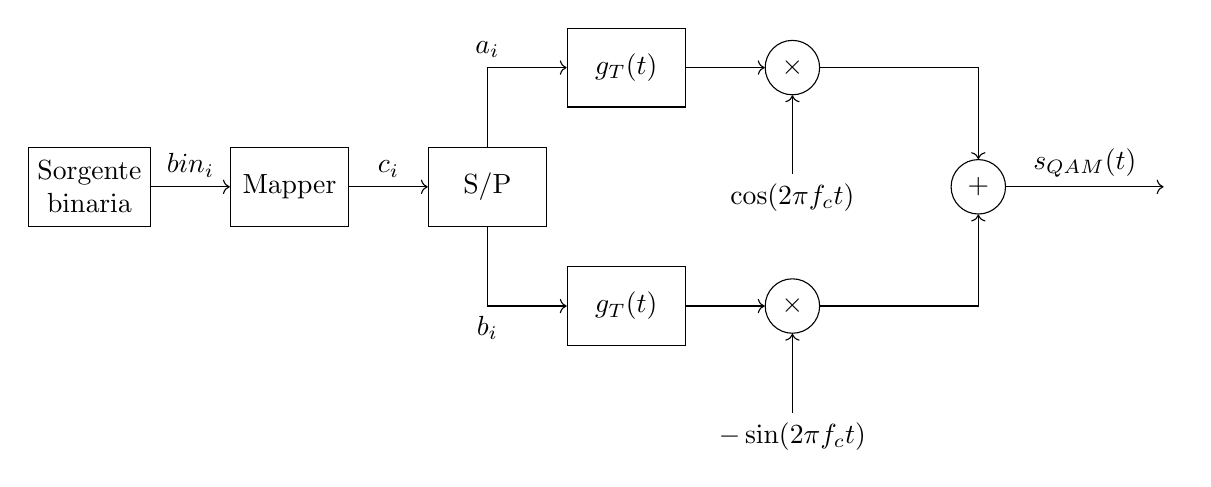
\begin{tikzpicture}[
            block/.style={rectangle, draw, minimum height=1cm, minimum width=1.5cm},
            node distance=1cm and 1cm,
            auto,
            every node/.style={align=center}
        ]
        % Blocks
        \node[block] (source) {Sorgente\\binaria};
        \node[block, right=of source] (encoder) {Mapper};
        \node[block, right=of encoder] (interp) {S/P};

        % create a node which is above interp
        \node[above=of interp, inner sep=0pt, minimum size=0pt] (dummy1) {};
        \node[below=of interp, inner sep=0pt, minimum size=0pt] (dummy2) {};


        \node[block, right=of dummy1] (p1) {$g_T(t)$};

        \node[block, right=of dummy2] (p2) {$g_T(t)$};
        \node[draw, circle, right=1cm of p1] (m1) {\(\times\)};
        \node[draw, circle, right=1cm of p2] (m2) {\(\times\)};

        \draw[->] (p1) -- (m1);
        \node[below=of m1] (cos) {$\cos(2\pi f_c t)$};
        \draw[->] (cos) -- (m1);

        \draw[->] (p2) -- (m2);
        \node[below=of m2] (sin) {$-\sin(2\pi f_c t)$};
        \draw[->] (sin) -- (m2);

        \node[right=2cm of m1, inner sep=0pt, minimum size=0pt] (dummy3) {};
        \node[right=2cm of m2, inner sep=0pt, minimum size=0pt] (dummy4) {};

        \node[draw, circle, right=5.125cm of interp] (sum) {\(+\)};

        \draw[->] (m1) -| (sum);
        \draw[->] (m2) -| (sum);

        \node[right=2cm of sum] (dummy5) {};
        \draw[->] (sum) -- node[midway, above] {$s_{QAM}(t)$} (dummy5) {};

        %\draw[-] (interp) -- (dummy1);
        %\draw[-] (dummy2) -- (interp);

        \draw[->] (interp) |- node[midway, above] {$a_i$} (p1);
        \draw[->] (interp) |- node[midway, below] {$b_i$} (p2);

        \draw[->] (source) -- (encoder) node[midway,above] {$bin_i$};
        \draw[->] (encoder) -- (interp) node[midway,above] {$c_i$};


    \end{tikzpicture}
\end{center}

La modulazione PAM non è utilizzata nella pratica perché non è molto efficiente dal punto di vista energetico.
Trasmettendo due PAM ortogonali si ottiene una modulazione QAM.
\[  
    s_{QAM}(t) = \underbrace{\sum_{i=-\infty}^{+\infty} a_i g_T(t - iT)}_{m_I} + j \underbrace{\sum_{i=-\infty}^{+\infty} b_i g_T(t - iT)}_{m_Q}
\]


I simboli trasmessi sono dunque complessi da un punto di vista matematico:

\[
    c_i = a_i + jb_i
\]

Che nella pratica equivale a due segnali PAM ortogonali.
Sfruttando la notazione complessa si ottiene:
\[
    s_{QAM}(t) = \sum_{i=-\infty}^{+\infty} c_i g_T(t - iT)
\]

La modulazione QAM essendo una combinazione di due PAM ortogonali con $M$ simboli prevede un totale di $M^2$ simboli. 







\begin{minipage}{.5\textwidth}
    \centering
    \begin{tikzpicture}
        \draw[->] (-4,0) -- (4,0) node[right] {$\Re$};
        \draw[->] (0,-4) -- (0,4) node[above] {$\Im$};

        \draw (0,1) -- (0.1,1) node[above] {$\ \ 1$};


        \foreach \point in {
                (-3, 1),
                (-3, -1),
                (3, 1),
                (3, -1),
                (-1, 1),
                (1, 1),
                (-1, -1),
                (1, -1)}{
                \draw[fill=orange] \point circle (1.5pt);
            }

        \node[below=4.5cm] at (0,0) {
            Simboli 8-QAM, $M_c = 4, M_s = 2$
        };

    \end{tikzpicture}

\end{minipage}
\noindent
\begin{minipage}{.5\textwidth}

    \centering
    \begin{tikzpicture}
        \draw[->] (-4,0) -- (4,0) node[right] {$\Re$};
        \draw[->] (0,-4) -- (0,4) node[above] {$\Im$};

        \draw (0,1) -- (0.1,1) node[above] {$\ \ 1$};


        \foreach \point in {
                (1, -3),
                (-1, -3),
                (1, 3),
                (-1, 3),
                (-1, 1),
                (1, 1),
                (-1, -1),
                (1, -1)}{
                \draw[fill=orange] \point circle (1.5pt);
            }


        % insert caption here
        \node[below=4.5cm] at (0,0) {
            Simboli 8-QAM, $M_c = 2, M_s = 4$
        };

    \end{tikzpicture}


\end{minipage}

I simboli possono essere quindi rappresentati nel piano complesso come in figura.

Considerando $M_c = M_s$, simboli indipendenti e a media nulla, il valor quadratico medio è:
\[
    A^{\text{QAM}} = \mathbb{E} \left\{  c_i c^*_i  \right\} = \mathbb{E} \left\{ a_i^2 \right\} + \mathbb{E} \left\{ b_i^2 \right\} = 2 \left( \frac{M^2 - 1}{3} \right)
\]

Mentre l'energia media per simbolo è:
\[
    E_s = \frac{A}{2} = \frac{M^2 - 1}{3}
\]

La probabilità di errore invece:
\begin{align*}
    x\left[ m \right] &= c_m + n \left[ m \right] \\
    &= a_m + j b_m + n_I \left[ m \right] + j n_Q \left[ m \right]
\end{align*}


L'evento di errore è $\mathcal{E}^{(i)} = \mathcal{E}_I^{(i)} \cup \mathcal{E}_Q^{(i)}$ quindi:
\[
    \mathbb{P} \left( e \mid c^{(i)} \right) = \mathbb{P} \left( \mathcal{E}^{(i)} \right) \leq \mathbb{P} \left( \mathcal{E}_I^{(i)} \right) + \mathbb{P} \left( \mathcal{E}_Q^{(i)} \right)
\]

ovvero:
\[
    P_e^{(M, QAM)} \leq 2 \ P_e^{(\sqrt{M}, PAM)}
\]
Facciamo quindi un'approssimazione che si chiama \textit{union bound}.




\[
\begin{array}{ccccc}
\text{4-QAM} & E_s = 1 = \frac{1}{\sigma} = \sqrt{\frac{E_s}{N_0}} & \Rightarrow & P_e^{\text{4-QAM}} < 2 \ Q\left(\sqrt{\frac{E_s}{N_0}}\right) \\
\text{16-QAM} & E_s = 5 = \frac{1}{\sigma} = \sqrt{\frac{E_s}{5N_0}} & \Rightarrow & P_e^{\text{16-QAM}} < 3 \ Q\left(\sqrt{\frac{E_s}{5N_0}}\right)\\
\end{array}
\]

Adesso le regioni associate a un simbolo sono porzioni del piano complesso, lungo 2 direzioni,
Per quanto riguarda l'errore sul bit, adottando la codifica di Gray, che vale quando abbiamo un SNR alto, si ottiene:
\[
    P_e^{(M-QAM, b)} = \lim_{N^{(b)} \to +\infty} \frac{N_e^{(b)}}{N^{(b)}} \approx \lim_{N^{(s)} \to +\infty} \frac{N_e^{(s)}}{\log_2(M) N^{(s)}} = \frac{1}{\log_2(M)} P_e^{(M-QAM)} 
\]

Sapendo che $P_e^{(M-QAM)} \leq 2 \ P_e^{(\sqrt{M}, PAM)}$ e che per la codifica di Gray $P_e^{(M-PAM, b)} \approx \frac{1}{\log_2{M}} P_e^{(M-PAM)}$ si ottiene:
\[
     P_e^{(M-QAM, b)} = \frac{1}{\log_2(M)} P_e^{(M-QAM)} \leq \frac{2}{\log_2(M)} P_e^{(\sqrt{M}, PAM)} = \frac{1}{\log_2(\sqrt{M})} P_e^{(\sqrt{M}, PAM)} \approx P_e^{(\sqrt{M}, PAM, b)}
\]

Da ciò si evince che la probabilità di errore sul bit per una QAM a $M$ simboli è approssimabile a quella di una modulazione PAM a $\sqrt{M}$ simboli.

